\chapter{Work Plan}\label{chap:work}

\section*{}

This chapter defines roughly the work plan for the next five months, in which
the research will be completed. Section~\ref{section:tasks} starts by defining
a major set of tasks, subsequently dividing each one into subtasks. It also
provides an estimated time for each one.

Then, in section~\ref{section:calendarisation}, these tasks are scheduled along
the next five months.

\section{Tasks}
\label{section:tasks}

In order to successfully employ an optimisation solution, I will develop a
simple framework for the evaluation of optimisation algorithms. This work has
already been started, but still needs some refinement. Once this is done, I
shall work on implement the optimisation techniques and develop the
architecture for communicating with the monitoring central system. I will also
compare these algorithms and provide benchmarks. As soon as these tasks are
done, I will focus on writing the thesis.

Next, I present a list with these tasks, their detailed description and an
estimated time. Figure~\ref{fig:gantt} shows a Gantt diagram with these tasks'
scheduling.

\begin{description}
\item[Framework] \hfill \\
Development of a framework for the evaluation and benchmark of optimisation
techniques. This involves finishing and polishing all modules described in
chapter~\ref{chap:approach}. This can be divided into the following subtasks:

\begin{itemize}
	\item Development of a tool that allows the editing of a city's containers and their fill rates;
	\item Implementation of the optimisation visualisation tool.
\end{itemize}

Estimated time: 4 weeks.

\item[Architecture] \hfill \\
Definition of an architecture for the communication between the optimisation
framework and the monitoring system.

\begin{itemize}
	\item Study of the current state on the fill status monitoring system;
	\item Design of a simple database to store information;
	\item Specify protocols for accessing and updating data.
\end{itemize}


Estimated time: 4 weeks.

\item[Optimisation] \hfill \\
Implementation and further study of different optimisation algorithms. This
requires the development of several heuristics, metaheuristics and exact methods
for both the \textit{commercial} and the \textit{rollon-rolloff} scenarios.

\begin{itemize}
	\item \textit{commercial} exact methods;
	\item \textit{commercial} heuristics;
	\item \textit{commercial} metaheuristics;
	\item adapt the \textit{commercial} approaches to the \textit{rollon-rolloff} scenario.
\end{itemize}

Estimated time: 8 weeks.

\item[Comparison] \hfill \\
Gathering of data to provide a solid comparison and benchmark of the
implemented algorithms. This task will also require parameter tuning and
sensibility analysis.


Estimated time: 4 weeks.

\item[Thesis writing] \hfill \\
Thesis writing, including a detailed documentation of the optimisation
techniques and their performance. Estimated time: 4 weeks.

\end{description}


\newpage
\section{Calendarisation}
\label{section:calendarisation}

Here, I present the calendarisation of the previously specified tasks.  Tasks
\textit{Framework} and \textit{Architecture} overlap because the framework will
eventually need to receive data from the fill status monitoring system.  Tasks
\textit{Architecture} and \textit{Optimisation} can be done interchangeably, as
they are independent. Finally, tasks \textit{Optimisation} and
\textit{Comparison} will slightly overlap because as the comparison between
techniques is done, further insight on their properties may provide clues to
their improvement.

\vspace{2cm}

\begin{figure}[th]
  \begin{center}
    \leavevmode

    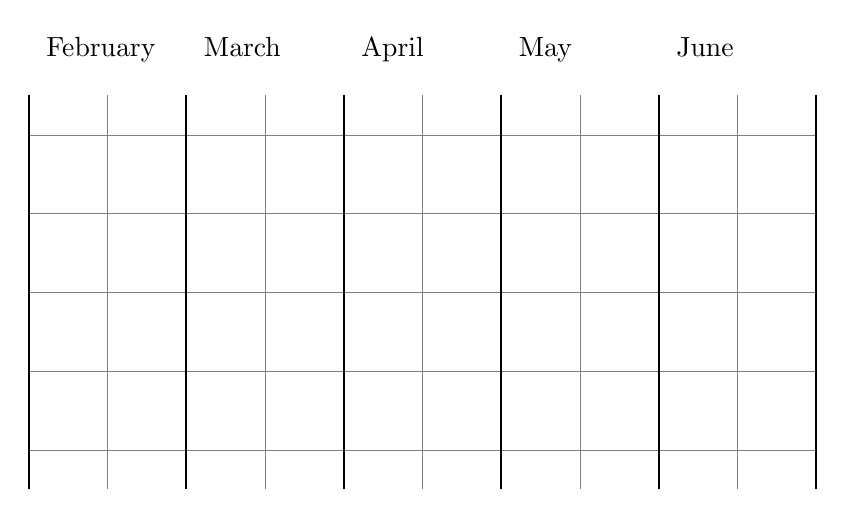
\begin{tikzpicture}[y=-1cm]
      \draw[help lines] (0,5.5) grid (10,0.5);
      \draw[thick] (0,0.5) -- (0,5.5);
      \draw[thick] (2,0.5) -- (2,5.5);
      \draw[thick] (4,0.5) -- (4,5.5);
      \draw[thick] (6,0.5) -- (6,5.5);
      \draw[thick] (8,0.5) -- (8,5.5);
      \draw[thick] (10,0.5) -- (10,5.5);
      
      \node at (0.1,0.0) [anchor=base west] {February};
      \node at (2.1,0.0) [anchor=base west] {March};
      \node at (4.1,0.0) [anchor=base west] {April};
      \node at (6.1,0.0) [anchor=base west] {May};
      \node at (8.1,0.0) [anchor=base west] {June};
      
      \ganttline{1}{Framework}{15}{45}
      \ganttline{2}{Architecture}{30}{60}
      \ganttline{3}{Optimisation}{45}{105}
      \ganttline{4}{Comparison}{75}{120}
      \ganttline{5}{Thesis Writing}{120}{150}
    \end{tikzpicture}

    \caption{Diagram containing the calendarisation of the tasks.}
    \label{fig:gantt}
  \end{center}
\end{figure}

